
% v2-acmsmall-sample.tex, dated March 6 2012
% This is a sample file for ACM small trim journals
%
% Compilation using 'acmsmall.cls' - version 1.3 (March 2012), Aptara Inc.
% (c) 2010 Association for Computing Machinery (ACM)
%
% Questions/Suggestions/Feedback should be addressed to => "acmtexsupport@aptaracorp.com".
% Users can also go through the FAQs available on the journal's submission webpage.
%
% Steps to compile: latex, bibtex, latex latex
%
% For tracking purposes => this is v1.3 - March 2012
\documentclass[prodmode,acmtecs]{acmsmall} % Aptara syntax
\usepackage[spanish,polish]{babel}
\usepackage[T1]{fontenc}
\usepackage{fancyvrb}
\usepackage{graphicx,hyperref}
\newcommand\cutout[1]{}


\usepackage[table]{xcolor}
\usepackage[utf8]{inputenc}
\usepackage[parfill]{parskip}
\usepackage{tabulary}
\PassOptionsToPackage{hyphens}{url}
\usepackage{hyperref}    
\usepackage[capitalize]{cleveref}


% Metadata Information
% !!! TODO: SET THESE VALUES !!!
\acmVolume{0}
\acmNumber{0}
\acmArticle{CFP}
\acmYear{0}
\acmMonth{0}

\newcounter{colstart}
\setcounter{page}{4}

\RecustomVerbatimCommand{\VerbatimInput}{VerbatimInput}%
{
%fontsize=\footnotesize,
fontfamily=\rmdefault
}


\newcommand{\UnderscoreCommands}{%\do\verbatiminput%
\do\citeNP \do\citeA \do\citeANP \do\citeN \do\shortcite%
\do\shortciteNP \do\shortciteA \do\shortciteANP \do\shortciteN%
\do\citeyear \do\citeyearNP%
}

\usepackage[strings]{underscore}



% Document starts
\begin{document}


\setcounter{colstart}{\thepage}

\acmArticle{CFP}
\title{{\huge\sc SIGLOG Monthly 258}

 February 2025}\author{ELLI ANASTASIADI\affil{Aalborg University, SE}\vspace*{-2.6cm}\begin{flushright}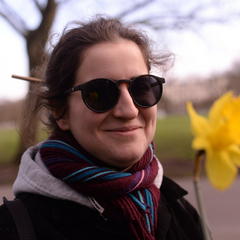
\includegraphics[width=30mm]{elli_anastasiadi.png}\end{flushright}}\begin{abstract}February 2025 edition of SIGLOG Monthly, featuring deadlines, calls and community announcements.
\end{abstract}


\maketitlee

\href{https://lics.siglog.org/newsletters/}{Past Issues}
 - 
\href{https://lics.siglog.org/newsletters/inst.html}{How to submit an announcement}
\section{Table of Contents}\begin{itemize}\item DEADLINES (\cref{deadlines}) 
 
\item CALLS 
 
\begin{itemize}\item ICALP 2025 (CALL FOR PAPERS) (\cref{ICALP2025})
\item ICLP 2025 (CALL FOR PAPERS ) (\cref{ICLP2025})
\item CSL 2025 (CALL FOR PARTICIPATION ) (\cref{CSL2025})
\item SSFT 2025 (CALL FOR PARTICIPATION) (\cref{SSFT2025})
\end{itemize} 
\end{itemize}\section{Deadlines}\label{deadlines}\rowcolors{1}{white}{gray!25}\begin{tabulary}{\linewidth}{LL}FMBC 1025:  & Feb 03, 2025 (Abstracts), Feb 10, 2025 (Full papers) \\
ICALP 2025:  & Feb 08, 2025 (Paper deadline) \\
FSCD 2025:  & Feb 10, 2025 (Abstracts), Feb 17, 2025 (Full papers) \\
LMW@CSL 2025:  & Feb 10, 2025 (On-site registration) \\
DEON 2025:  & Mar 01, 2025 (Abstract deadline), Mar 08, 2025 (Paper deadline) \\
SSFT 2025:  & Mar 31, 2025 (Registration of applications) \\
CONCUR 2025:  & Apr 01, 2025 (Abstract deadline), Apr 07, 2025 (Paper deadline) \\
ICLP 2025:  & Apr 13, 2025 (Paper registration (regular papers)), Apr 18, 2025 (Paper  (regular papers)), Jun 15, 2025 (Paper  (short papers)) \\
\end{tabulary}
\section{ICALP 2025: 52nd EATCS International Colloquium on Automata, Languages, and Programming}\label{ICALP2025}  Aarhus, Denmark, July 8-11, 2025\\ 
  \href{https://conferences.au.dk/icalp2025}{https://conferences.au.dk/icalp2025}\\ 
CALL FOR PAPERS 

\begin{itemize}\item  ICALP is the main conference and annual meeting of the European Association for Theoretical Computer Science (EATCS). As usual, ICALP will be preceded by a series of workshops, which will take place on July 7. The 2025 edition has the following features: 
 
\begin{itemize}\item  Submissions are anonymous and there is a rebuttal phase.
\item  The conference is planned as a physical, in-person event.
\end{itemize} 
\item  IMPORTANT DATES (AoE) 
 
\rowcolors{1}{white}{gray!25}\begin{tabulary}{\linewidth}{LL}Paper deadline:  & Feb 08, 2025 \\
Rebuttal:  & Mar 21, 2025 \\
Author notification:  & Apr 14, 2025 \\
Camera-ready version:  & Apr 28, 2025 \\
Early registration:  & TBA \\
Workshops July 7, 2025:  &  \\
Conference:  & Jul 8-11, 2025 \\
\end{tabulary}
 
  Deadlines are firm; late submissions will not be considered. 
 
\item  INVITED SPEAKERS   
 
\begin{itemize}\item  Anupam Gupta - NYU, USA
\item  Mary Wootters - Stanford University, USA
\item  Hongseok Yang - KAIST, Korea
\item  One or two more speakers TBC
\end{itemize} 
\item  WORKSHOPS  
 
  On Monday 7 July, the following workshops will take place: 
 
\begin{itemize}\item  Fair Allocations
\item  Loop Invariants and Algebraic Reasoning
\item  Theory and Applications of Algorithms with Predictions
\item  Algorithmic Aspects of Temporal Graphs
\item  Graph Width Parameters
\end{itemize} 
\item  AWARDS  
 
  During the conference, the following awards will be delivered: 
 
\begin{itemize}\item  the EATCS award,
\item  the Presburger award,
\item  the EATCS distinguished dissertation award,
\item  the best papers for Track A and Track B,
\item  the best student papers for Track A and Track B.
\end{itemize} 
\item  GUIDELINES 
 
  Submissions to ICALP 2025 use HotCRP system: Submission server Track A: \href{https://icalp25-a.hotcrp.com}{https://icalp25-a.hotcrp.com} . Submission server Track B: \href{https://icalp25-b.hotcrp.com}{https://icalp25-b.hotcrp.com} 
 
\begin{itemize}\item   Papers must present original research on the theory of computer science. No prior publication and no simultaneous submission to other publication outlets (either a conference or a journal) is allowed. Authors are encouraged to also make full versions of their submissions freely accessible in an on-line repository such as ArXiv, HAL, ECCC.
\item  Submissions take the form of an extended abstract of no more than 15 pages, excluding references and a clearly labelled appendix. The appendix may consist either of omitted proofs or of a full version of the submission, and it will be read at the discretion of program committee members. The use of the LIPIcs document class is an option, but not required. The extended abstract has to present the merits of the paper and its main contributions clearly, and describe the key concepts and technical ideas used to obtain the results. Submissions must provide the proofs which can enable the main mathematical claims of the paper to be verified.
\item   Submissions are anonymous. The conference will employ a lightweight double-blind reviewing process. Submissions should not reveal the identity of the authors in any way. Authors should ensure that any references to their own related work are in the third person (e.g., not “We build on our previous work …” but rather “We build on the work of …”). The purpose of this double-blind process is to help PC members and external reviewers come to an initial judgment about the paper without bias, and not to make it impossible for them to discover who the authors are if they were to try. Nothing should be done in the name of anonymity that weakens the submission or makes the job of reviewing the paper more difficult. In particular, important references should not be omitted. In addition, authors should feel free to disseminate their ideas or draft versions of their paper as they normally would. For example, authors may post drafts of their papers on the web, submit them to arXiv, and give talks on their research ideas.
\item  Submissions authored or co-authored by members of the program committee are allowed.
\item  The submissions are done via HotCRP to the appropriate track of the conference. The use of pdflatex or similar pdf generating tools is mandatory and the page limit is strict (see point 2.) Papers that deviate significantly from these requirements risk rejection without consideration of merit.
\item  During the rebuttal phase, authors will have from March 21-24, 2025 the opportunity to view and respond to initial reviews. Further instructions will be sent to authors of submitted papers before that time.
\item  At least one author of each accepted paper is expected to register for the conference, and all talks are in-person. In exceptional cases, there may be support for remotely presenting a talk.
\item  Papers authored only by students should be marked as such upon submission in order to be eligible for the best student paper awards of the track.
\end{itemize} 
\item  PROCEEDINGS  
 
  ICALP proceedings are published in the Leibniz International Proceedings in Informatics (LIPIcs) series. This is a series of high-quality conference proceedings across all fields in informatics established in cooperation with Schloss Dagstuhl – Leibniz Center for Informatics. LIPIcs volumes are published according to the principle of Open Access, i.e., they are available online and free of charge. The accepted papers will need to comply with the LIPIcs style. 
 
\end{itemize}\section{ICLP 2025: 41st International Conference on Logic Programming }\label{ICLP2025}  University of Calabria, Rende, Italy | September 12-19, 2025\\ 
  \href{https://iclp25.demacs.unical.it/}{https://iclp25.demacs.unical.it/}\\ 
CALL FOR PAPERS  

\begin{itemize}\item  SCOPE 
 
  Since the first conference In Marseille in 1982, ICLP has been the premier international event for presenting research in logic programming. Contributions are sought in all areas of logic programming, including but not restricted to:  
 
\begin{itemize}\item  Theoretical Foundations: Formal and operational semantics, Non-monotonic reasoning, Reasoning under uncertainty, Knowledge representation, Semantic issues of combining logic and neural models, Complexity results.
\item  Language Design and Programming Methodologies: Concurrency and parallelism, Mobility, Interacting with ML, Logic-based domain-specific languages, Hybrid logical and imperative/functional languages, Programming techniques, Answer Set Programming, Inductive Logic Programming, Coinductive Logic Programming
\item  Program Analysis and Optimization: Analysis, Transformation, Verification, Debugging, Profiling, Visualization, Logic-based validation of generated programs.
\item  Implementation Methodologies: Compilation, Parallel/distributed execution, Constraint implementation, Tabling, Logic-based prompt engineering, User interfaces.
\end{itemize} 
\item  IMPORTANT DATES (TENTATIVE): 
 
\rowcolors{1}{white}{gray!25}\begin{tabulary}{\linewidth}{LL}Paper registration (regular papers):  & Apr 13, 2025 \\
Paper submission (regular papers):  & Apr 18, 2025 \\
Notification to authors (regular papers):  & May 25, 2025 \\
Paper submission (short papers):  & Jun 15, 2025 \\
Revision submission (regular papers):  & Jun 15, 2025 \\
Final notification to authors:  & Jul 06, 2025 \\
Main conference:  & Sep 15-19, 2025 \\
\end{tabulary}
 
  Paper submission will be through EasyChair, following the link \href{https://easychair.org/conferences/?conf=iclp25}{https://easychair.org/conferences/?conf=iclp25}.   
 
  Accepted regular papers will appear in the journal Theory and Practice of Logic Programming (TPLP). Accepted short papers will be published by Electronic Proceedings in Theoretical Computer Science (EPTCS). The respective paper formats are described at: 
 
\begin{itemize}\item  \href{https://www.cambridge.org/core/journals/theory-and-practice-of-logic-programming/information/instructions-contributors}{https://www.cambridge.org/core/journals/theory-and-practice-of-logic-programming/information/instructions-contributors}
\item  \href{http://style.eptcs.org/}{http://style.eptcs.org/}
\end{itemize} 
\item  AFFILIATED EVENTS: 
 
\begin{itemize}\item  Workshops: September 12-14, 2025
\item  Doctoral Consortium: September 12-14, 2025
\item  Autumn School in Computational Logic: September 12-14, 2025
\item  Thematic Tracks (to be announced)
\item  International Symposium on Principles and Practice of Declarative Programming (PPDP 2025)
\item  Logic-based Program Synthesis and Transformation (LOPSTR 2025)
\end{itemize} 
\item  VENUE: 
 
  ICLP’25 will be held on the campus of the University of Calabria in Rende, Italy, in September 2025. The University of Calabria is one of Italy's leading academic institutions, renowned for its innovative research and vibrant campus life. Located in the scenic city of Rende, it offers a modern learning environment surrounded by natural beauty and cultural richness. Calabria is a region rich in culture, offering a blend of historical heritage and stunning natural beauty. From its breathtaking coastal spots to its easily accessible mountains, the region provides an unforgettable cultural and culinary experience, savoring authentic dishes made from fresh, local ingredients, such as spicy 'nduja, pasta, potatoes and exquisite desserts. 
 
\item  ORGANIZATION: 
 
\begin{itemize}\item  General Chair: Francesco Ricca
\item  Program Co-chairs: Daniela Inclezan and Martin Gebser
\item  Publicity Chairs: Manuel Borroto and Francesco Calimeri
\item  Local Chairs: Antonio Ielo and Giuseppe Mazzotta
\end{itemize} 
\end{itemize}\section{CSL 2025: 33rd EACSL Annual Conference on Computer Science Logic }\label{CSL2025}  10-14 February 2025, Amsterdam, the Netherlands\\ 
  \href{https://csl2025.github.io/index}{https://csl2025.github.io/index}\\ 
CALL FOR PARTICIPATION  

\begin{itemize}\item  ABOUT  
 
  CSL is the annual conference of the European Association for Computer Science Logic (EACSL). It is an interdisciplinary conference, spanning across both basic and application oriented research in mathematical logic and computer science. CSL 2025 will be held on the 10th–14th of February 2025 and is organised jointly by the Theoretical Computer Science group at the Vrije Universiteit Amsterdam and ILLC at the University of Amsterdam. 
 
\item  CO-LOCATED WORKSHOPS  
 
  Two workshops are co-located with CSL, and will take place on Monday, February 10: 
 
\begin{itemize}\item  12th Logic Mentoring Workshop (LMW@CSL 2025)
\item  Workshop on Learning and Logic (LeaLog@CSL 2025)
\end{itemize} 
\item  REGISTRATION  
 
  Late registration, from January 11 up to and including February 5 is: regular fee 820 euro, student fee 505 euro, only workshop 75 euro. After February 5, only onsite registration is possible: regular fee 970 euro, student fee 605 euro, only workshop 75 euro. The registration form can be found at: \href{https://fd20.formdesk.com/vu-onlinepayment/Beta_Registration_form_CSL_2025}{https://fd20.formdesk.com/vu-onlinepayment/Beta\_Registration\_form\_CSL\_2025} . The registration fee includes the welcome reception, lunches, and the conference excursion and dinner. The student fee for CSL 2025includes LMW and LeaLog and an annual 5 euro EACSL membership fee. 
 
  Please indicate (in the allergies field) if you intend to attend a workshop, and if so, which one (or both). If you want to register for one of the (or both) workshops, please select the LMW option of 50 euro, and indicate (in the allergies field) which workshop(s) you will attend. This registration fee includes free attendance of the CSL 2025 welcome reception on Monday afternoon. 
 
\begin{itemize}\item  dh Early Registration: Feb 10, 2025
\end{itemize} 
\end{itemize}\section{SSFT 2025: Fourteenth Summer School on Formal Techniques}\label{SSFT2025}  Atherton, California, May 24-30, 2025\\ 
  \href{https://SSFT-SRI.github.io}{https://SSFT-SRI.github.io}\\ 
  Menlo College, Atherton, California\\ 
CALL FOR PARTICIPATION 

\begin{itemize}\item  Techniques based on formal logic, such as model checking, satisfiability, static analysis, and automated theorem proving, are finding a broad range of applications in modeling, analysis, verification, and synthesis. This school, the fourteenth in the series, focuses on the principles and practice of formal techniques, with a strong emphasis on the hands-on use and development of this technology. It primarily targets graduate students and young researchers who are interested in studying and using formal techniques in their research. A prior background in formal methods is helpful but not required. Participants at the school can expect to have a seriously fun time experimenting with the tools and techniques presented in the lectures during the laboratory sessions. The main lectures run from Monday May 26 to Fri May 30. They are preceded by a background course ``Speaking Logic'' on May 24/25. 
 
\item  The lecturers at  the school include: 
 
\begin{itemize}\item  Joost-Pieter Katoen (RWTH Aachen): Deductive Verification of Probabilistic Programs with Caesar
\item  Erika Abraham (RWTH Aachen): Understanding and using SAT and SMT solvers
\item  Kristin Yvonne Rozier (Iowa State): Runtime Verification with R2U2
\item  Philippa Gardner (Imperial): Compositional Verification using the Gillian Platform
\item  Nate Foster (Cornell University): Programming and Reasoning with Kleene Algebra with Tests
\end{itemize} 
  The program also features invited talks from distinguished speakers (to be announced) and the background ``Speaking Logic'' course taught by Natarajan Shankar (SRI) and Stephane Graham-Lengrand (SRI). 
 
\item  The 2025 Summer School on Formal Techniques will take place in a hybrid mode: the lectures and labs will be live-streamed and recorded. We strongly encourage in-person participation so that you can benefit from interactions outside the classroom. We have funding from NSF to cover transportation/food/lodging expenses for selected US-based students. Non-student and non-US in-person participants are expected to cover their own transportation and will be charged a fee (around $150/day) to cover the cost of food and lodging. The registration link is at the URL: \href{https://SSFT-SRI.github.io}{https://SSFT-SRI.github.io}. 
 
  Applicants are urged to submit their applications as early as possible (no later than March 31, 2025), since there are only a limited number of spaces available. Those needing invitation letters for visa purposes should complete their applications as early as possible.  We strongly encourage the participation of women and under-represented minorities in the summer school. 
 
Registration of applications: Mar 31, 2025 
 
\end{itemize}


\bigskip Links: \href{http://siglog.org/}{SIGLOG website}, \href{https://lics.siglog.org}{LICS website}, \href{https://lics.siglog.org/newsletters/}{SIGLOG Monthly}\end{document}